%PART_2_CHAP_2
\myChapter{C}{hoix de l'architecture}
%WAIT a Review ok
\begin{resumChap}[.8]
Ce deuxième chapitre a pour objet de présenter les constituants historiques de la plate-forme Poppy à savoir son architecture open source \tiret{tant sur les matériels que sur les software} qui a permis la création d'une communauté autour de différents usages. En premier lieu pour la science puis pour les arts et les makers en tous genres. À cette communauté se greffent rapidement d'autres usages, d'autres objectifs: l'éducation des sciences du numérique au travers de la robotique.\par%
Ce chapitre sera également l'occasion de présenter plus en détails les caractéristiques techniques du Kit robotique ErgoJr. Chacune de ces caractéristiques découle d'un choix de conception qui sera explicité. Nous aborderons donc d'abord les caractéristiques hardware, puis software et enfin les caractéristiques des ressources pédagogiques associées, à savoir:le site web, le forum et les activités type.
\end{resumChap}
\section{L'existant, la plateforme Poppy}\label{sec:poppy}
    \nociteUrl{poppy-project, poppy-Education, poppy-forum, poppy-doc, poppy-crowdin, poppy-source, poppy-source-pypot, poppy-source-ergo, poppy-ProjectTwitter, poppy-EduTwitter, poppy-Youtube, poppy-Vimeo, poppy-Flickr, poppy-3D, poppy-userMap, poppy-distrib}
    L'un des aspects essentiels du projet Poppy est de pouvoir le modifier pour l'adapter à son contexte d'utilisation. Ainsi toute personne peut créer son Poppy possédant ses caractéristiques propres. Poppy Humanoïde est distribué aujourd'hui sous forme de kit à monter soi-même, tout comme ses déclinaisons \cro{standards}: PoppyTorso et ErgoJr. 
    Sur le modèle original, les proportions du corps ont été 'bio-inspirées', car il était destiné à étudier la marche bipède humaine.
    Poppy, comme tous les robots, utilise ses effecteurs pour modifier son environnement en conséquence des retours sensoriels de ses capteurs. Il agit en fonction des différentes commandes et algorithmes qui lui ont été implantés. Les comportements pré-enregistrés sont appelés primitives, d'un point de vue conceptuel ces comportements par défaut peuvent être considérés comme la partie relevant de l'inné.
    \begin{figure}[!h]
        \centering
        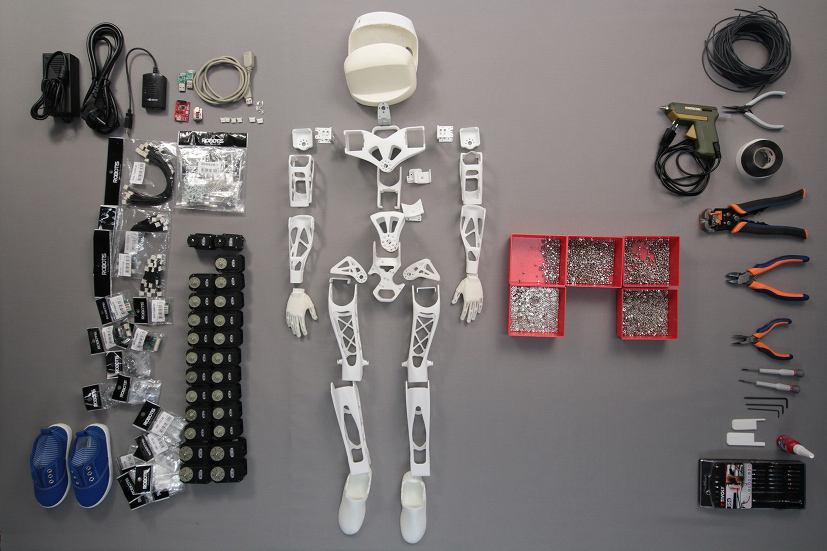
\includegraphics[width=0.45\linewidth]{Figures/poppy_components}
        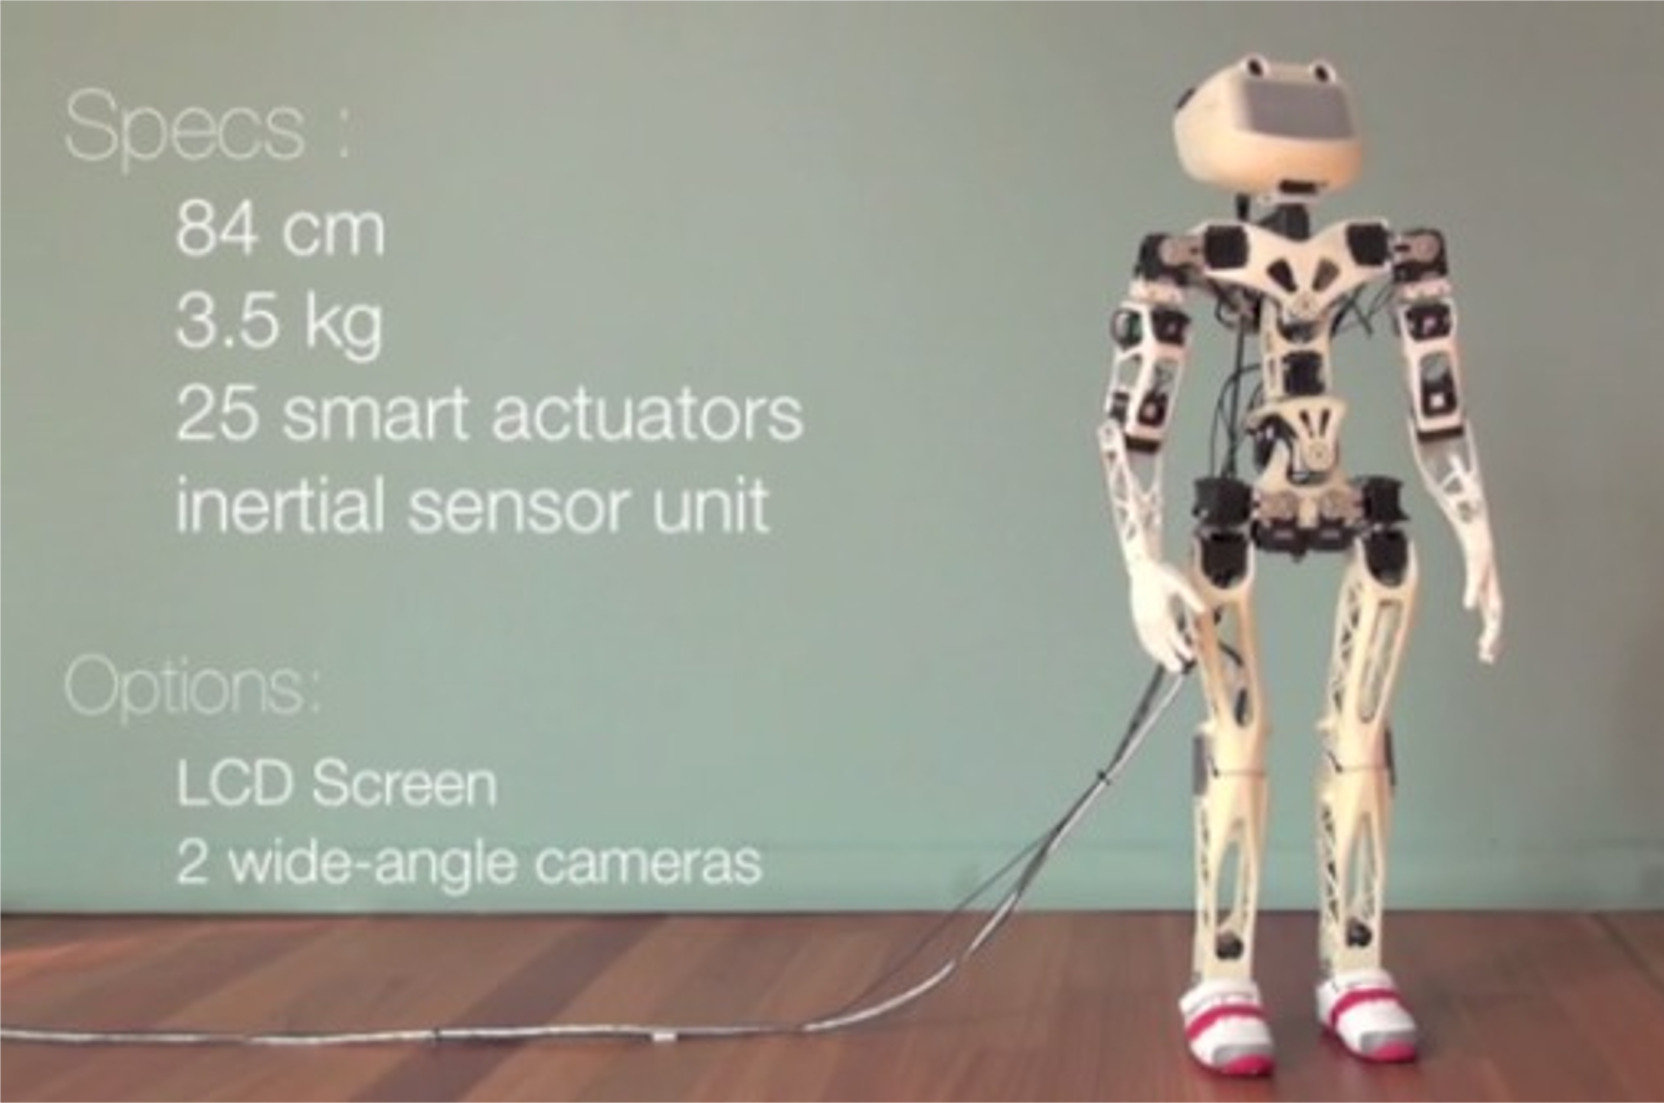
\includegraphics[width=0.45\linewidth]{Figures/poppy_spec}
        \caption{Composants Poppy Humanoïde}
        \label{fig:poppy_spec}
    \end{figure}\par%
    Poppy Humanoïde est composé de 25 moteurs. Le coût de ces moteurs rend cette plateforme onéreuse,les autres composants sont moins onéreux. Un seul servo-moteur coûte environ 250\euro{} soit 25 x 250\euro{} = 6250\euro{} pour un coût total de 8350\euro{} TTC. Réduire ce coût fût l'une des principales raisons qui a conduit à l'élaboration de PoppyTorso, ayant 12 moteurs de moins (soit 5150\euro{} TTC), et surtout à l'élaboration d'une nouvelle plateforme lowcost: ErgoJr.
    Ceci a été possible car l'ensemble des parties plastiques sont facilement modifiables via un modèle de \sht{CAO}, puis par sa fabrication grâce à l'impression 3D.
    Il faut noter que cette technologie est de plus en plus accessible: dans les lycées, les écoles supérieures, les \sht{fablab}, à la maison, \etc~\citeS{sec:3D_print}.
    Ce qui unit tous les robots Poppy est, non pas leur morphologie, mais d'une part leur idéologie: des robots modifiables et open-source permettant la reproductibilité des résultats; et d'autre part leur modalité de contrôle: la partie software.\par%
    Toutes les ressources accessibles du projet sont disponibles sur ces différents sites~\citeT{tab:poppy_link}, dépendant de l'usage et des informations qu'on recherche.
    \begin{table}[!h]
        \centering
        \begin{sc}
        \begin{tabular}{| l | p{5.9cm}|}
            \hline
            Siteweb Poppy-project~\citeURL{poppy-project}                    & \url{https://www.poppy-project.org} \\ \hline
            Siteweb dédié à l'éducation~\citeURL{poppy-Education}            & \url{https://www.poppy-Éducation.org} \\ \hline
            Forum (support et community discussions)~\citeURL{poppy-forum}   & \url{https://forum.poppy-project.org} \\ \hline
            Documentation en ligne~\citeURL{poppy-doc}                       & \url{https://docs.poppy-project.org} \\ \hline    
            Pypot code source~\citeURL{poppy-source}                         & \url{https://github.com/poppy-project/pypot} \\
            \hline
            Poppy ErgoJr code source~\citeURL{poppy-source-ergo}             & \url{https://github.com/poppy-project/poppy-ergo-jr} \\ 
            \hline
            Distributeur Poppy Robot~\citeURL{poppy-distrib}                 & \url{https://www.generationrobots.com/} \\ \hline
        \end{tabular}
        \end{sc}
        \caption{Principaux liens Web}
        \label{tab:poppy_link}
    \end{table}\par%
    La richesse du Kit ErgoJr vient également de la communauté Poppy Éducation (enseignants, élèves, développeurs, passionnés de robotique, \dots), qui l’enrichit continuellement, grâce à diverses contributions et collaborations. Nous avons déjà rappelé le rôle et l'importance de la communauté et de ses outils de communication dans un projet open-source~\citeS{sec:com-open}, nous présenterons la manière dont la communauté Poppy Éducation s'est construite et développée.
    \subsection{Pour la science}\label{sec:poppy_science}
        En 2012, Matthieu Lapeyre a débuté une thèse dans le but d’explorer le rôle de l’incarnation et des propriétés morphologiques sur la cognition et en particulier l’apprentissage de tâches sensori-motrices. À cette époque, aucune des plateformes existantes ne répondait aux besoins liés à la nécessité de diffuser et de pouvoir reproduire des expériences dans un contexte de recherche à un coût abordable.
        \begin{figure}[!h]
        \begin{minipage}{0.475\linewidth}
            \centering
            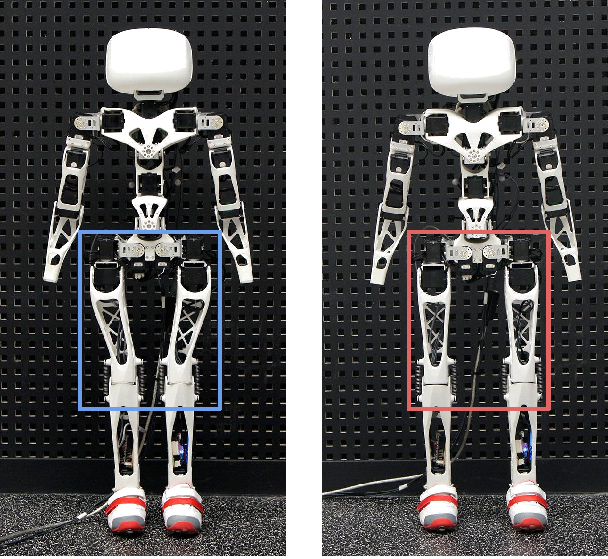
\includegraphics[width=0.975\linewidth]{Figures/poppy_legs}
            \caption{Poppy, relation morphologie et équilibration~\citeB{lapeyre2013poppy}}
            \label{fig:poppy_legs}
        \end{minipage}
        \hfill
        \begin{minipage}{0.5\linewidth}
        \myDefautStyle
            Ces besoins ont donné naissance à un ensemble d'outils formant une plateforme de création robotique, et un premier robot a été conçu en 2014 avec cette plateforme: Poppy, qui a été rebaptisé Poppy-project.
            L'un des tout premiers travaux réalisé par M.Lapeyre \& P.Rouanet~\citeB{lapeyre2013poppy} concepteurs de Poppy, portait sur l'équilibration. Plus particulièrement sur la chute  (vitesse \& vélocité) en fonction de l'agencement morphologique des jambes.%~\citeF{fig:poppy_legs}.
        \end{minipage}
        \end{figure}\par%
        Pour faciliter le développement du \textit{Poppy-project}, des outils numériques ont été mis en place: Par exemple, la plateforme GitHub~\citeURL{poppy-source} a été choisie pour que chacun puisse accéder à toutes les ressources du projet et proposer des modifications.
        Le projet a également choisi comme habitat numérique un forum de discussions (Discourse)~\citeURL{poppy-forum}, et c'est, à ce jour, la plateforme sur laquelle sont faites les annonces importantes. En ce qui concerne le site web~\citeURL{poppy-project}, Wordpress a été choisi: un outil de gestion de contenu avec un bon support, une interface très intuitive pour les non-initiés au développement web et des thèmes prêts à l'emploi peu coûteux.
        Des contenus multimédias consacrés à Poppy-project ont été proposés sur les sites dédiés au projet ainsi que sur les réseaux sociaux (YouTube~\citeURL{poppy-Youtube}, Twitter~\citeURL{poppy-ProjectTwitter}, Flickr~\citeURL{poppy-Flickr}, Vimeo~\citeURL{poppy-Vimeo}), afin de donner une vision d'ensemble de tout ce que pouvait apporter la plateforme. L’équipe du projet a également été très active en participant à de nombreux événements, salons, colloques, formations, et en veillant à une interactivité significative dans le forum Poppy, où les utilisateurs de la plateforme étaient encouragés à s’exprimer et à échanger, ce qui a fortement développé la communauté des usagers de Poppy. Cette conjugaison des qualités intrinsèques de Poppy avec sa diffusion dans les médias, amplifiée par le bouche à oreille, a rapidement apporté une grande visibilité au projet.
        Cette animation du forum, la présence de Poppy sur les réseaux et dans les événements liés à l’éducation et à la robotique, s’est accrue au fur et à mesure de la diversification des usages de Poppy.
    \subsection{Pour tous}
        A ses débuts, Poppy était principalement axé sur la recherche puis utilisé pour les arts chorégraphiques, pour l’enseignement supérieur, et dans les FabLabs. La plateforme s’est ensuite avérée, d'après certains utilisateurs, être un formidable outil pour l’enseignement des sciences du numérique dans l’enseignement secondaire et pour des projets artistiques originaux (à partir de l’école maternelle, avec la mise en mouvement de l’humanoïde).
        Pour se développer, la communauté Poppy Éducation s'est appuyée sur la communauté Poppy-project, %cette dernière étant celle de la plateforme robotique Poppy dont est issu le robot Poppy ErgoJr.
        En effet, de cette communauté est née une communauté plus petite et plus spécifique mais partageant un intérêt global pour l'écosystème Poppy. La communauté Poppy Éducation a notamment bénéficié de l'architecture de participation et de la notoriété liée à la campagne de promotion sur le terrain du Poppy-project, ce qui a été un atout mais également un défi, dans le sens où il a fallu adapter la structure et le mode de fonctionnement aux besoins spécifiques de cette communauté pour créer une identité propre. Par exemple, la communauté Poppy-project cible un large public (scientifiques, techniques, artistiques et éducatifs) principalement anglophones et technophiles (développeurs, bidouilleurs, hobbyist, \etc) alors que Poppy Éducation cible majoritairement un public francophone et de débutants (enseignants, élèves, grand public, \etc). Il a alors fallu adapter les outils et en développer de nouveaux, pour finalement aboutir à deux communautés différentes qui interagissent. Cette spécialisation progressive de la communauté en communautés thématiques utilisant un outil commun est un phénomène global pour le Poppy-project.
        \begin{figure}[!h]
            \centering
            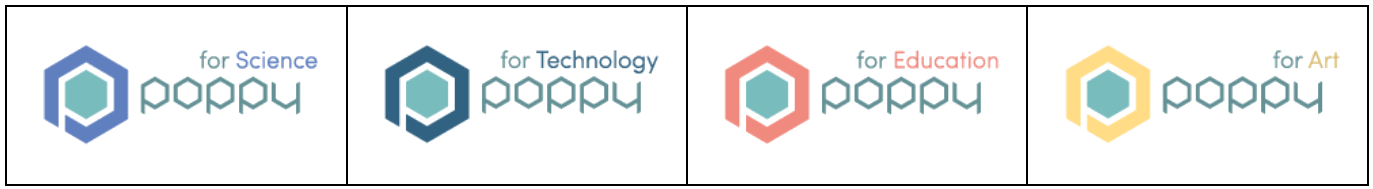
\includegraphics[width=\linewidth]{Figures/Poppy-BlocMarques}
            \caption[Identité graphique Poppy-project]{Identité graphique des différentes sphères thématiques du projet Poppy}
            \label{fig:blocmarque}
        \end{figure}\par%
        \paragraph{Pour les artistes}
            ErgoJr s'inspire du tout premier modèle des robots Poppy, qui à l'origine n'était qu'un bras articulé composé de 6 moteurs reliés par des pièces métalliques: Ergo-Robot (aujourd'hui appelé Poppy~ErgoSr). C'est cette version qui avait été utilisée par P-Y.Oudeyer dans ses recherches sur la curiosité et le langage~\citeB{oudeyer2011curiosity}. Suite aux résultats, une démonstration du setup expérimental a eu lieu en continu durant plusieurs jours au sein de la Fondation Cartier à Paris en 2011, afin de mettre en avant la nécessité d'utiliser des modèles d'apprentissages artificiels devant s'incarner dans une enveloppe robotique tangible et non simulée.
            \begin{figure}[!h]
                \centering
                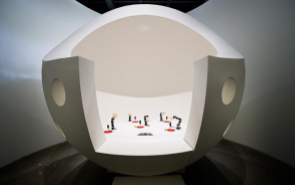
\includegraphics[width=0.45\linewidth]{Figures/Oudeyer_expo-cartier}
                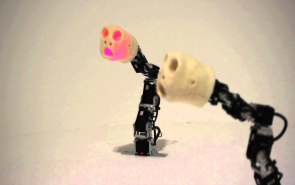
\includegraphics[width=0.45\linewidth]{Figures/Poppy_Ergo-lynch}
                \caption{Exposition à la fondation Cartier}
                \label{fig:expo_ergo}
            \end{figure}\par%
            Un autre projet avec les Poppy humanoïdes cette fois, consistait en une résidence d'artistes intitulée \gui{Êtres et Numériques}. Dirigée par les artistes Amandine Braconnier (artiste technique mixte) et Marie-Aline Villard (danseuse-chercheuse), soutenue par le Fabrik Pola et l'Aquitaine Régie, ce projet d'art contemporain s'est concentré sur la manière d'exprimer des émotions par le mouvement robotique du corps dans \gui{action avec un danseur humain}. Ce travail a pris la forme d'une résidence de sept jours en sciences et arts impliquant des membres du projet Poppy et des artistes. 
            S'en est suivi d'autres résidences puis d'autres collaborations~\citeB{villard2016mouv}, nous pouvons notamment citer un cours de danse en 2\ieme année de Licence~\citeS{sec:villard_cours}; où le projet mené avec canopé: \gui{Poppy entre dans la danse}~\citeS{sec:canope_danse}.
            La communauté d'artistes est une source d'inspiration riche et peut offrir de nouvelles perspectives aux questions scientifiques et technologiques. Cette complémentarité est une grande opportunité que nous souhaitons mettre en œuvre dans le projet Poppy en rendant le robot accessible aux utilisateurs non-experts en robotique.
            Aujourd'hui cet art se retrouve avec des actions comme la participation à la robocup junior dans la catégorie \cro{on stage} avec le robot ErgoJr~\citeS{sec:on-stage} ou plus simplement dans le storietelling de certaines activités~\citeS{sec:activite}.
        \paragraph{Pour les enseignants}
            La plateforme Poppy a fortement suscité l'intérêt du domaine de l'éducation, non seulement pour des projets de robotique dans les écoles d'ingénieurs, mais aussi pour initier les élèves de lycée aux sciences du numérique. L'équipe s'est alors rapprochée des enseignants de l'ancienne Région Aquitaine pour discuter de ce qu'il serait possible de faire avec la plateforme Poppy. Il se trouve que le robot Poppy ErgoJr répondait bien aux besoins des établissements scolaires. L'équipe Poppy s'est dotée de spécialistes en pédagogie qui ont lancé ce nouveau projet par une campagne de prêt de robots. Ainsi, Poppy Éducation était né. Dans ce domaine, la vie de la communauté est encore plus importante sur le terrain: lors de la création du projet, c'est le contact avec les enseignants de l'ancienne Région Aquitaine qui a favorisé le développement de cette communauté. L'accompagnement à l'usage des robots dans les classes était nécessaire. Un fois que les utilisateurs se sont appropriés les robots, la communauté a pu se développer largement sur le web. Plusieurs exemples de parcours d'appropriation par les enseignants seront traités plus loin~\citeS{sec:entretiens}.
        \paragraph{Pour les \textit{Makers}}\label{sec:makers}
            Cette partie de la communauté est celle dont nous avons le moins d'information car beaucoup plus autonome. La majeure partie des interactions s'effectue directement sur le github. Les sujets principaux de conversation concernent des sujets techniques ou précis.
            La grande majorité des individus inclus dans cette communauté reste tout simplement anonyme. Ainsi aucune de leurs réalisations ou productions n'est visible par les autres membres de la communauté.
            Cependant, certains individus de cette communauté documentent, partagent et diffusent leurs travaux comme par exemple avec Julien Jhel et son site web Roboticia~\citeURL{roboticia}
            \myPhantom{subparagraph}{Julien Jhel}
                En 2015 Julien Jhel définissait l'objectif de mettre sur son site l’ensemble de la documentation et des ressources pédagogiques pour qu’un enseignant non spécialiste de l’informatique puisse utiliser la plateforme Poppy dans ses cours. Un an plus tard, il ouvrait une \sht{SAS}. Aujourd'hui, Roboticia se définit comme \gui{une société spécialisée dans la conception de robots et d’objets connectés. Robotic-I-A réunie la mécatronique et l’intelligence artificielle pour fabriquer des objets intelligents. Nos robots éducatifs sont open-source et nous fournissons donc des briques à tous ceux qui veulent pratiquer le DIY (Do It Yourself). Nous fournissons aussi du contenu pédagogique}.%\par%
            \myPhantom{subparagraph}{Thomas Peyruse}
                Un autre cas notable est celui de Thomas Peyruse, dit \textit{Thot} sur le Forum Poppy qu'il a rejoint en Mars 2014 et où il y est aujourd'hui modérateur. De formation d'ingénieur en aéronautique, c'est dans le cadre d'une reconversion professionnelle vers les arts qu'il a connu le projet Poppy. Il se définit aujourd'hui, entre autres, comme un artiste roboticien au sein de la compagnie Shonen~\citeURL{shonen} et comme un artiste numérique au sein de l'association Caliban Midi~\citeURL{caliban}. Par ailleurs, il propose son expertise pour des événements de divertissement autour de la robotique, ainsi que de conférences au travers de son auto-entreprise \gui{marionnettes électriques}~\citeURL{marionnettes}. Il a également co-fondé la société KONEXinc~\citeURL{konex} spécialisée dans la domotique et l'analyse (locale) des traces de smarthome.
        \paragraph{User-map}\label{sec:map}
            Une tentative de recensement a été initiée afin de mieux visualiser l'étendue de la communauté, aussi bien en terme de volume qu'en terme de localisation. Pour cela, nous avons sélectionné la solution \textit{umap} proposée par \textit{Open Street Map} et avons ajouté les utilisateurs connus~\citeURL{poppy-userMap}. Nous avons ensuite posté un lien sur le forum, pour que tout nouvel utilisateur puisse s'enregistrer directement sur la carte. Cependant, peu de nouveaux utilisateurs ont effectué cette démarche.
    \subsection{Code source}\label{sec:code_source}
        \begin{figure}[!h]
        \begin{minipage}{0.45\linewidth}
            \centering
            \href{https://docs.poppy-project.org/}{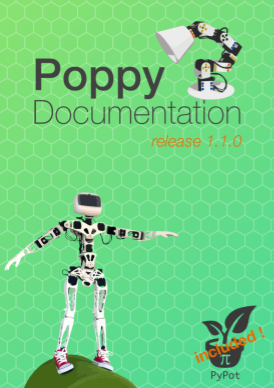
\includegraphics[width=0.85\linewidth]{Figures/Poppy-doc}}
            \caption{Documentation Poppy}\label{fig:poppy_doc}
        \end{minipage}
        \hfill
        \begin{minipage}{0.545\linewidth}
            \centering
            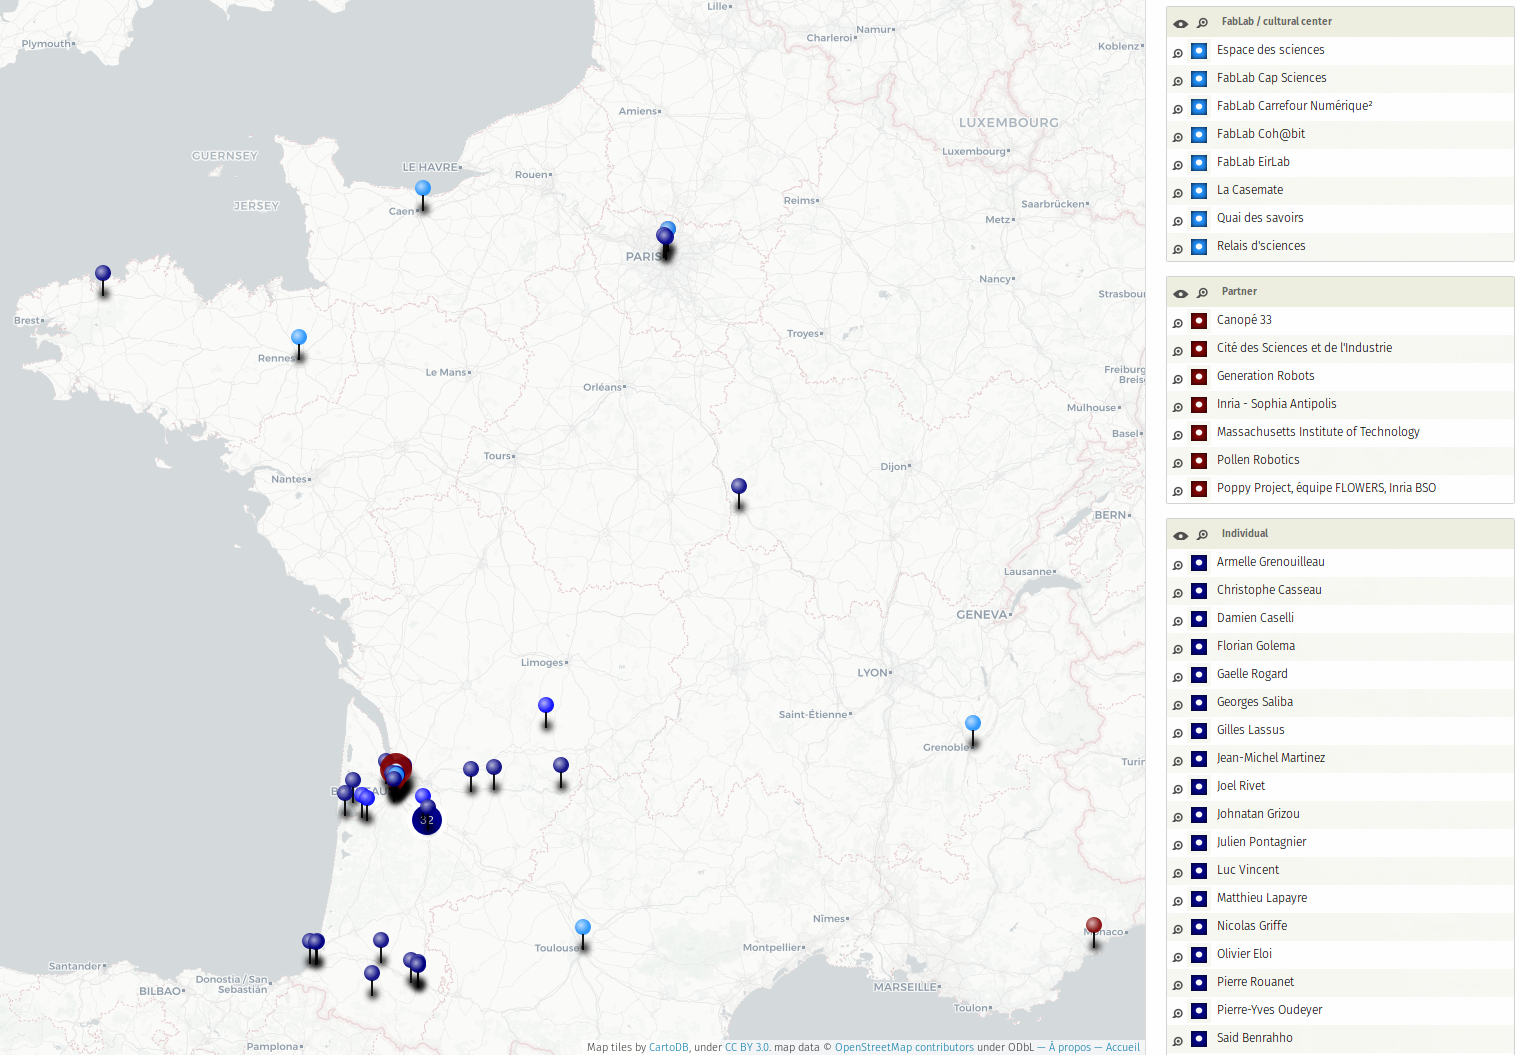
\includegraphics[width=\linewidth]{Figures/poppy-umap.png}
            \caption{Poppy Users Map}\label{fig:poppy_map}
        \end{minipage}
        \end{figure}\par%
        La documentation~\citeURL{poppy-doc} du projet se veut la plus abordable possible pour les différents types de public qui peuvent s'y intéresser.
        Elle a été construite en utilisant gitbook, un générateur de site statique à partir d'une syntaxe markdown, spécifiquement conçu pour des documentations.
        La documentation est hébergée sur un \href{https://github.com/poppy-project/poppy-docs}{dépôt git}~\citeURL{poppy-source}, elle est compilée automatiquement à chaque contribution et le site se met à jour quelques minutes plus tard.
        Elle est rédigée en anglais sur lequel se base une traduction française complète (et partielle en espagnol). La  traduction est faite à l'aide de \href{https://crowdin.com/project/poppy-docs/fr}{crowdin}~\citeURL{poppy-crowdin}, un outil permettant de faire de la traduction collaborative, permettant de gérer efficacement les mises à jour des traductions en fonction des mises à jour des sources.
\section{Robot Poppy ErgoJr}
    Le Projet Poppy Éducation s’appuie sur le robot Poppy ErgoJr pour ses expérimentations.
    Ce robot a été conçu à l'aide de la plate-forme Poppy, qui se compose d'un ensemble d’outils logiciels et matériels permettant la création et la modification de robots. Nous allons les détailler dans cette partie et expliquer les choix qui ont amené à leur utilisation.\par%
    La forme et les déplacements du robot sont intimement liés à son interaction avec l'environnement. Le robot, pour pouvoir réaliser certaines actions et se déplacer, a besoin de détecter et connaître certains éléments sur son environnement et sur lui-même. Ceci est assuré par des capteurs d'éléments externes et internes. Là où les capteurs permettent de récupérer de l'information sur l'environnement, le robot doit également pouvoir agir sur cet environnement. Ces actions sont réalisées grâce à des actionneurs, des émetteurs et autres composants permettant de modifier l'environnement et le robot lui-même.% a replacer ?
    C'est sa programmation contenue dans son micro-contrôleur qui permettra de déterminer quelles actions effectuer en fonction des captations réalisées. De cette interaction avec l'environnement émerge le comportement du robot.
    \subsection{Hardware}
        \subsubsection{Micro-contrôleur}
            Une question fréquemment posée concerne le choix d'un ordinateur embarqué type Raspberry~Pi plutôt qu'une carte basée sur un micro-contrôleur de type Arduino. Ce choix s'explique en partie pour des raisons techniques, historiques.
            Le robot ErgoJr fait partie du projet Poppy. Ces robots partagent les mêmes briques logicielles, et les mêmes idées de conception. ErgoJr a été conçu en s'inspirant fortement de Poppy Humanoid et de Poppy Torso.
            Utiliser un ordinateur embarqué comme la Raspberry~Pi possède de nombreux avantages. Cela permet d'utiliser un système d'exploitation et des fonctionnalités et programmes qui y sont disponibles. Ceci permet l'utilisation facile de programmes complexes \textit{multi-threadés} et de fonctionnalités au niveau du contrôle des moteurs et des mouvements qui seraient beaucoup plus difficiles à faire sur un micro-contrôleur.
            \begin{figure}[!h]
                \centering\label{fig:Hardware}
                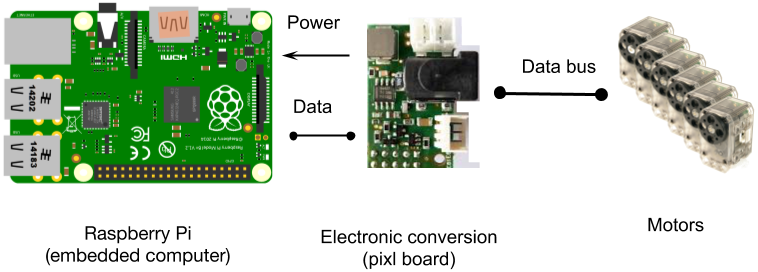
\includegraphics[width=0.9\linewidth]{Figures/Segonds-hardware_robot.png}
                \caption{Architecture Hardware, Segonds~\cite{RI}}
            \end{figure}\par%
            Aussi, la Raspberry~Pi permet d'embarquer tous les logiciels nécessaires pour programmer le robot, il suffit de se connecter à l'interface web et on a accès a \sht{snap}, Jupyter pour la programmation en Python, \etc. D'un point de vue logiciel et en dehors du contrôle strict des moteurs, avoir un système d'exploitation permet de bénéficier de plein de librairies logicielles perfectionnées, qui sont utiles pour certains utilisateurs. Par exemple on utilise OpenCV pour faire du traitement d'image. Ce serait impossible sur un micro-contrôleur de type Arduino, tant en terme de ressources de calculs que de possibilités de l'architecture.
            Cependant, il faut noter que le développement au sein d'un laboratoire de recherche est souvent accès sur la facilité d'itération et de modification plutôt que sur le coût d'un produit fini. Utiliser un micro-contrôleur permet de baisser les coûts, mais c'est au prix d'un développement plus compliqué, pour obtenir des résultats similaires.
            Il serait possible d'embarquer un micro-contrôleur sur le robot ErgoJr et de déporter une partie de la complexité (traitement d'image par exemple) sur le périphérique client (ordinateur, tablette). Cette architecture est très fréquente aujourd'hui dans la robotique éducative 
            Du fait des contraintes du matériel informatique et du réseau de l'enseignement secondaire public~\citeS{sec:materiel}, disposer d'un robot qui nécessite le moins possible d'installer ou de modifier quoi que ce soit grâce à son interface web est un atout important.
        \subsubsection{Capteurs et Effecteurs}
            Les capteurs d'un robot sont séparables en deux catégories, ceux externes qui visent à capter l'environnement qui entoure le robot, et ceux internes qui visent à récupérer des informations sur l'état du robot.
            \paragraph{Capteurs externe: la caméra}
                {Le kit ErgoJr est muni d’une caméra, cette dernière permet de détecter l’environnement externe. Le programme de contrôle du robot étant développé sous Python~\citeS{sec:code_source}, qui est installé sur la Raspberry~Pi, l'intérêt est ici porté sur les librairies disponibles pour le traitement d’images dans ce langage car c'est elles qui détermineront \textit{in fine} les capacités (caractéristiques) du matériel utilisé, ici une caméra~PI~2.0.
                Il existe en Python deux principales librairies pour le traitement d’images.
                La librairie Python Imaging Library (PIL), développée depuis 1995, elle ne dispose plus de mises à jour depuis 2011. Mais un fork créé par la suite, qui se nomme Pillow, permet de réaliser des manipulations basiques d’images et continue à être développé.
                La deuxième librairie principale est Open Computer Vision (OpenCV). C'est une bibliothèque graphique libre développée depuis 2000 (son support est actuellement assuré par Intel). Elle possède en particulier des outils avancés de traitement d’images, de vidéos et des algorithmes d’apprentissages classiques. Elle est disponible sous C++, Python et Java. Elle est largement utilisée dans le monde de la recherche du fait de ses nombreuses fonctionnalités.
                OpenCV a de nombreux avantages face à Pillow, il dispose de plus nombreuses fonctionnalités, plus avancées, en particulier pour le traitement de vidéos. OpenCV est également plus rapide pour des tâches égales (en moyenne trois à quatre fois plus rapide)~\citeURL{pil_vs_OCV}. Mais en contrepartie, OpenCV est plus lourd que Pillow.
                Ainsi, il convient plutôt d’utiliser Pillow si l’on a besoin uniquement de fonctions de traitement d’images et qu'il est nécessaire d'avoir quelque chose de léger. Dans le cadre du projet, il y a un potentiel besoin d’analyse de vidéos en temps réel, OpenCV est donc plus adapté.}%%%
                À noter que par défaut, ErgoJr reconnaît 4 cartes schématiques ressemblant à des QR codes. Un code documenté en ligne permet de générer ses propres cartes~\citeURL{GS-QRcode}.
            \paragraph{Capteurs additionnels}
                Il existe d'autres capteurs externes qui auraient pu être intéressants à utiliser: capteurs tactiles, capteurs de proximité, capteurs de distance. Cependant, chaque ajout représente un coût pour le kit final qui se devait de rester le plus bas possible. Malgré cela, la possibilité de \gui{upgrade} le kit reste possible. Ainsi prenons l'exemple de l'activité ErgoJr plays TicTacToe~\citeS{sec:prof-GL} qui utilise par le biais de Arduino des capteurs photosensibles afin de détecter la présence des jetons sur la grille. Ou plus simplement l'ajout d'une caméra usb déportée sur le côté pour analyser une partie précise de l'espace~\citeF{fig:tic-tac-toe}.% note sur octave delorme ?
            \paragraph{Servomoteur}
                \myPhantom{subparagraph}{Définition}
                    Tout d'abord, les servomoteurs ne sont pas de simples moteurs. Ils contiennent également des engrenages permettant d'augmenter le couple du moteur, un encodeur et un circuit de contrôle qui permettent de maintenir une position, \etc.
                   ~\citeAtion{servo}
                \subparagraph{Le choix pour ErgoJr}
                    Le kit ErgoJr est un kit permettant de construire son propre robot à bas coût. C'est pourquoi les servomoteurs utilisés dans ce kit ne doivent pas avoir un prix trop important.
                    Ainsi, les servomoteurs choisis sont les XL-320. Ils ont la possibilité d'être branchés les uns à la suite des autres afin de faciliter l'assemblage de petits robots. Ils sont légers (16.7g) et font partie des servomoteurs à bas coût (autour de 22 euros pièce). %peuvent appliquer un couple de 3.98 kg.cm. Ils
                    En comparaison, pour le même ordre de prix, il existe également le servomoteur Hitec HS-485HB, mais il a un poids bien plus important (45g).% et un couple plus important également (4.8kg.cm).
                    Nous pouvons également citer le servomoteur à rotation continue de Futaba, mais qui lui aussi reste relativement lourd (45g)%Il pèse également 45g et a un couple de 3.4kg.cm.
                    Le XL-320 a donc l'avantage d'être léger et d'avoir malgré tout un couple satisfaisant. De plus, la possibilité d'en brancher plusieurs en série est utile lors de la fabrication d'un bras robotique. Cependant, son poids le rend plus fragile, ce qu'il faut prendre en compte lors de la conception par des mécanismes logiciels empêchant d'aller au delà de certaines limites angulaires par exemple.
                    En outre, afin d'utiliser facilement des servomoteurs, des librairies sont nécessaires. Elles permettent de parler au servomoteur sans avoir à coder de nouveau des fonctions usuelles et sans avoir a se préoccuper de quel signal envoyer, à quelle fréquence et pendant combien de temps. Une librairie populaire est «servo», qui est une librairie d'Arduino. Elle permet de contrôler jusqu'à 12 servomoteurs (avec la carte Arduino).
                    Concernant Poppy, une autre librairie a été développée dans le langage Python, conçue spécialement pour les servomoteurs Dynamixel: la librairie PyPot~\citeS{sec:pypot}. C'est celle-ci qui fut réutilisée pour l'implémentassion de ErgoJr.
                \subparagraph{Dynamixel XL-320}
                    Les robots Poppy utilisent donc comme actionneurs des moteurs Dynamixel.
                    Ces moteurs ont la particularité d'être connectés en réseau les uns aux autres de façon chaînée.  Ils communiquent par liaison série asynchrone Half Duplex: ils communiquent sur le même canal de communication (appelé bus de données). Ils peuvent également renvoyer des informations à l'utilisateur.
                    Chacun des moteurs est identifié de façon unique sur le bus de données par un identifiant reconfigurable stocké dans sa mémoire interne.
                    Cet identifiant est ensuite associé logiciellement à un nom correspondant à l'emplacement physique d'un moteur dans le robot.
                    Connecter les moteurs de façon chaînée un à un plutôt que chacun à la carte de contrôle -comme c'est le cas avec des servomoteurs classiques- permet de réduire la longueur des câbles, de faciliter leur passage et leur branchement pour l'utilisateur.
                    En plus de pouvoir répondre à des commandes de position angulaire, comme c'est uniquement le cas avec des servomoteurs classiques, ceux-ci peuvent se commander également en vitesse et en couple. De plus il est possible de modifier les paramètres du contrôleur P.I.D de l'asservissement du moteur ce qui permet d'ajuster la vitesse et la souplesse de la réponse, et de l'adapter à des cas d'utilisations précis.
                    Ils font aussi office de capteurs, en renvoyant à la demande leur position actuelle, leur vitesse, leur couple (pour détecter si la pince est fermée sur un objet ou non par exemple), leur température et leur tension d'alimentation.
                    Sur le robot ErgoJr, les moteurs sont reliés à la Raspberry~Pi par la carte pixl -pixl pour Rasberry\textbf{pi-XL}320% les XL-320 étant le nom des moteurs Dynamixel.
                    Cette carte permet d’alimenter la Raspberry~Pi à partir de l’alimentation des moteurs (leur tension nominale étant différente) et de faire la conversion entre le protocole de communication des moteurs (TTL 5V half duplex) et l'interface de communication de la Raspberry~Pi (UART 3.3V).
            \paragraph{Autres effecteurs}    
                {Grâce à sa capacité à capter son environnement, un robot peut agir dessus en fonction de son but. Il existe plusieurs moyens pour un robot de réaliser des actions sur son environnement. Le premier moyen est par le biais de ses membres qui sont souvent actionnés par des moteurs. Par exemple, actionner une pince pour qu'elle attrape des objets~\citeURL{LV-cafe}. Il en existe bien davantage, notamment grâce à du son ou de la lumière qui lui permettent une autre forme d'interaction avec l'utilisateur:
                les moteurs utilisés dans le kit ErgoJr possèdent 3 LEDs de couleurs programmables, une de chaque couleur élémentaire (rouge, bleue, verte). L'association des trois permettant de faire afficher une couleur comme le jaune par exemple. En pratique, cela donne une possibilité d'afficher 8 couleurs différentes. Étant donné qu'un ErgoJr possède 6 moteurs, cela lui donne un nombre important de combinaisons possibles. Les LEDs peuvent, par exemple faire passer un message suivant un code couleur, en indiquant que si une des LEDs d'un moteur s'allume en rouge, c'est que le moteur surchauffe.
                Dans plusieurs activités, un code couleur est notamment mis en place pour visualiser le \cro{mode d'intéraction} des moteurs \eg rouge=stiff vert=complient~\citeS{sec:activite}
                Il est aussi possible de brancher des écouteurs ou des enceintes à la Raspberry~Pi grâce à sa prise jack. Cela donne la possibilité, par exemple, de faire parler le robot ou encore d'émettre des sons ou de la musique.}%%%
        \subsubsection{Forme}
            Pour éviter tout à priori dépendant d'éléments culturels, nous avons choisi de faire un robot qui ressemble à un objet du quotidien. Inoffensif, inutile même de premier abord, un robot en forme de lampe de bureau n'évoque pas grand chose lorsqu'il est inanimé, l'attente est donc faible, contrairement à une forme anthropomorphique ou zoomorphique qui suscitera une forte attente en terme de capacité d'action~\citeS{sec:forme}.
            L'attente est faible, le robot ne sait rien faire sans l'implication de l'élève, mais il est facile de lui faire se mouvoir. L'utilisateur est donc acteur, il n'y a pas de magie, pas d'intelligence projetée dans cet objet, mais un engagement venant de la curiosité et du progrès ressentis par l'élève dans le contrôle du robot.
            De plus, le robot ErgoJr est livré en pièces détachées, une étape de montage d'une heure est nécessaire à son utilisation. Cette étape est importante pour l'engagement de l'élève, elle crée un lien entre le robot et l'élève, lui donnant un sentiment de l'avoir fabriqué.
            Il existe un très grand nombre de robots pédagogiques à roues: Thymio, mBot, Ozobot, Bee-bot, Finch, \etc~\citeS{sec:bot}, ne nécessitant seulement que deux moteurs pour un grand nombre d'interactions possibles, cela semble un bon compromis entre le coût et les possibilités offertes. Cependant, les activités pédagogiques  qui en découlent sont assez répétitives entre ces différents robots, il est difficile de trouver des activités qui soient originales. Pour cela, nous avons fait le choix de nous orienter vers une forme moins répandue, un bras manipulateur fixe.
            Les pièces sont conçues avec Onshape, un logiciel de modélisation paramétrique 3D. Il est facile à utiliser, gratuit pour des projets publics, possède de nombreux tutoriels et il fonctionne dans un navigateur web.
            Il propose des fonctionnalités avancées pour la collaboration telles que le partage de pièces créées pour s'en servir de base pour de nouveaux projets, l'édition d'une même pièce à plusieurs, simultanément, ou encore un gestionnaire de version similaire à ce qui existe pour gérer du code chez les développeurs.
            Cela permet de favoriser la création et la modification des pièces par la communauté d'utilisateurs.
            L'utilisation de l'impression 3D permet, par rapport, à l'injection plastique des coûts de lancement de production plus faibles, la production de moules de qualité industrielle étant très onéreuse.
            Ceci permet également aux étudiants, aux enseignants et aux bidouilleurs de créer facilement leurs propres pièces ou d'adapter des pièces existantes afin d'obtenir le robot qu'ils souhaitent. Ce phénomène est exacerbé par l'arrivée de nouveaux outils à visée pédagogique tels que TinkerCad et des moyens de diffusion associés tel que thingivers%citeURL
            Enfin les pièces mécaniques sont reliées aux moteurs à l'aide de petits rivets en plastique (rivets Ollo), permettant de monter, d'enlever ou de changer une pièce rapidement. Pour les utiliser, il faut se servir d'un outil de la forme d'un petit pied de biche (un Ollo tool), mais de nombreux enfants le font directement avec les doigts, ce qui en illustre la simplicité d'utilisation.
    \subsection{Software}
        \paragraph{Bas niveau}\label{sec:pypot}
            %cf Pierre rouanet 
            Les robots sont contrôlés par la bibliothèque logicielle pypot ainsi qu'une autre bibliothèque portant le nom du robot et spécifique à celui-ci servant à spécifier sa configuration et ses comportements dédiés.
            Pypot est une librairie Python développée comme un framework au sein de l'équipe Inria FLOWERS pour permettre de contrôler facilement et rapidement des robots constitués de moteurs Dynamixel.
            Pypot est centrale dans la plate-forme Poppy. Elle permet de faire l’interface avec le protocole de communication des moteurs, de définir des comportements (\cro{Primitives}) qui seront synchronisés entre eux avec un système d’orchestration, de fournir une API HTTP permettant de s’interfacer avec d’autres langages, de se connecter à des simulateurs pour contrôler de façon indifférenciée un robot tangible et une version simulée.
        \paragraph{Web App}
            %cf Theo Segonds
            L'avantage le plus évident de l'utilisation d'une interface web pour contrôler le robot est qu'il n'y a rien à télécharger. Il suffit d'ouvrir un navigateur web -sans même nécessiter internet- pour accéder à la programmation. Ceci rend le déploiement des robots dans des classes où les enseignants n'ont pas les droits administrateurs sur les ordinateurs beaucoup plus facile.
            La seule dépendance à un navigateur, rend aussi l'utilisation du robot immédiatement possible sur tout périphérique ayant un navigateur web moderne. L'utilisation des tablettes ou de chromebook étant répandue dans les classes en France (mais pas rencontrée dans notre étude), cela constitue un nouvel avantage.
            \begin{figure}[!h]
                \centering
                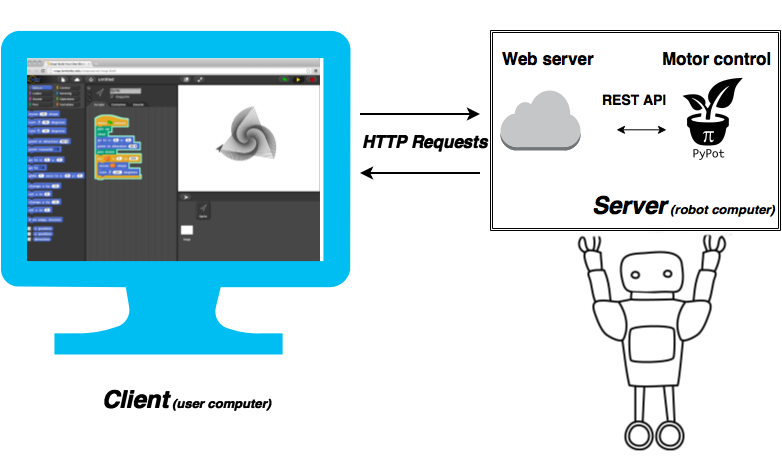
\includegraphics[width=0.9\linewidth]{Figures/Segonds-web_app}
                \caption{Architecture WebApp, Seguonds \cite{RI}}\label{fig:WebApp}
            \end{figure}\par%
            Cependant, l'utilisation d'un navigateur pour programmer à aussi des inconvénients. Les navigateurs web installés dans les classes peuvent ne pas être à jour, et le support des dernières normes HTML5/CSS3 n'est pas toujours bon sur de vielles versions. De plus, \sht{snap} effectue le rendu des blocs avec l'élément HTML \textit{canvas}, dont le support de l'accélération matérielle peut varier beaucoup d'un navigateur et d'un système d'exploitation à l'autre. Ainsi, le projet de base de \sht{snap} pour l'utilisation du robot comprend de nombreux blocs, et il arrive que des ordinateurs disposant d'un chipset graphique peu puissant mettent plusieurs dizaines de secondes à charger la page. De façon générale les navigateurs basés sur le moteur web \textit{Blink} (Chromium, Opera), sont nettement plus rapides à afficher les blocs \sht{snap} que ceux basés sur \textit{Gecko} (Firefox).
            L'utilisation d'un navigateur web pour contrôler le robot va de pair avec le fait que le robot et l'ordinateur de l'étudiant sont connectés sur le même réseau. Dans une salle de classe, il est ainsi fréquent que tous les ordinateurs et robots soient sur le même réseau. Cela peut poser un \textit{problème} au début, où les élèves vont s'amuser à contrôler les robots les uns des autres, mais rapidement cela devient une fonctionnalité pédagogique intéressante. Par exemple, en cas d'un faible nombre de robots, les élèves peuvent travailler avec le simulateur et chacun leur tour, lancer leur code sur le robot présent sur la table de l'enseignant en changeant uniquement le contenu de la variable \textit{host} dans le projet \sht{snap}. Cela permet aussi de façon triviale de lancer des commandes sur plusieurs robots en même temps, depuis un même \sht{snap} et ainsi de réaliser des projets complexes comprenant plusieurs robots collaborant pour une même tâche.%DNS
        \paragraph{Modèle numérique}
            \begin{figure}[!h]
            \begin{minipage}{0.495\linewidth}
                \centering
                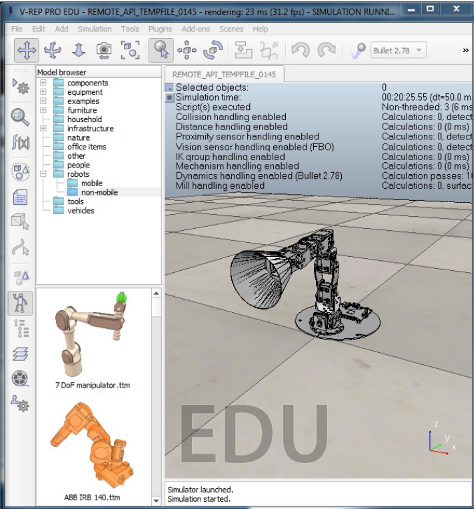
\includegraphics[width=\linewidth]{Figures/Poppy-ErgoJr_simu}
                \subcaption{Simulation V-Rep, Rouanet~\cite{RI}}
            \end{minipage}\hfill
            \begin{minipage}{0.48\linewidth}
                \centering
                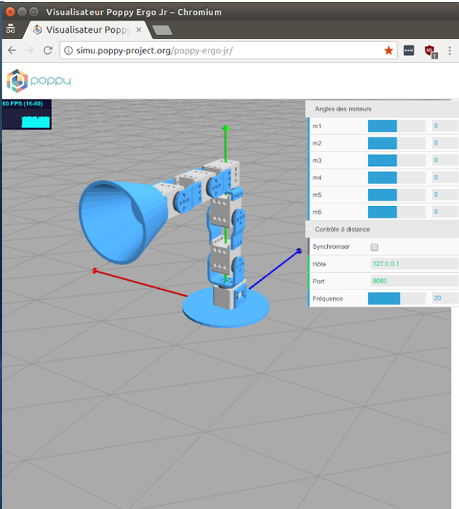
\includegraphics[width=\linewidth]{Figures/Poppy-ErgoJr_visu}
                \subcaption{Visualisation WebGL, Caselli~\cite{RI}}
            \end{minipage}
            \caption[Deux objets virtuels: une simulation et une visualisation]{Deux objets virtuels}
            \label{fig:visu_simu}
            \end{figure}\par%
            Avoir une version numérique des différentes créatures proposées par la plate-forme Poppy semblait être une nécessité~\citeS{sec:devellopement}. De plus, {il est courant d’avoir recours à des visualiseurs 3D afin de se représenter le robot en cours de développement, et d’étudier son comportement au sein d’une simulation physique, ce qui permet, lors de la conception de nouveaux algorithmes, de réaliser des premiers tests de manière rapide et sure, sans risquer d’endommager le vrai robot parfois onéreux.
            Il existe donc de nombreux logiciels permettant de créer un robot (en terme de structures, articulations, capteurs, programmes\dots) et de le visualiser au sein d’un environnement pouvant être doté d’une physique plus ou moins fidèle à la réalité.}%%%
            \myPhantom{subparagraph}{Simulation}
                {De longue date existait une version simulée du Poppy humanoide, portée sur un logiciel dédié nommé V-REP. Une entrée dans le code source Pypot a permis d'interfacer les fonctionnalités du robot  avec l'API de V-REP (acceptant du code LUA). 
                Une comparaison détaillée de V-REP~\citeB{pitonakova2018feature} à deux autres simulateurs open-sources répandus, Gazebo et ArGoS, montre que  V-REP est un simulateur plus complexe et gourmand en ressources, ce qui peut le rendre désavantageux si l’on cherche à simuler le comportement de plusieurs robots en même temps. Cependant, V-REP permet de modéliser de nouveaux robots de manière très détaillée, et de les faire évoluer dans un environnement à la physique développée.}%%%
                De plus, son implémentassion était déjà effectuée et une scène intégrant le robot Torso et une autre scène intégrant le robot ErgoJr ont simplement été ajoutées. 
                Côté utilisateur, V-REP est à installer sur son ordinateur et propose une version gratuite pour l'éducation. Un moteur physique y est intégré permettant d'ajouter des objets soumis à la gravité.
            \myPhantom{subparagraph}{Visualisation}
                D'un autre côté, une version plus simple a été développée: celle-ci ne nécessitant aucune installation préalable: elle s'exécute directement dans le navigateur web de l'ordinateur. Elle permet de visualiser le robot, cependant aucun ajout d'objet ni aucune gestion de la gravité n'y est directement proposé. Cet outil est à considérer comme un complément et non comme une alternative à une simulation V-REP.
            \myPhantom{subparagraph}{Gratuité}
                La possibilité de pouvoir tester gratuitement des outils qui restent aujourd'hui onéreux semble une formidable opportunité pour les utilisateurs. Cependant, il ne faut pas négliger que l'une des caractéristiques principales de ces outils est leur caractère tangible. Or, utiliser une version numérique de ces outils leur fait perdre cette caractéristique intrinsèque et on peut se demander légitimement s'il n'y a pas un décalage entre leurs tests et les attentes qu'ils suscitent, avec la réalité de l'outil robotique une fois en main. De plus, nous pouvons constater que certains enseignants utilisent ces versions numériques directement dans leurs enseignements. Bien évidemment, ils adaptent le contenu pédagogique à l'objet qu'ils manipulent. Cependant, pouvons-nous constater une différence significative dans certains contextes favorisant une version réelle~\citeS{Exp:Reel_virtuel}, auquel cas nous pourrions nous demander si utiliser une version numérique d'un outil robotique est suffisant pour justifier son utilisation ou si, au contraire, une version réelle est nécessaire voir indispensable. 
        \paragraph{Connectivité}
            Les établissements scolaires ont une architecture réseau ainsi que du matériel et logiciel hétérogènes~\citeS{sec:connect_classe}. La connexion au robot dans ces conditions est un élément crucial pour l'adoption du robot.
            Pour répondre à ces différentes problématiques, nous nous sommes tournés vers un ordinateur embarqué -une Raspberry~Pi- qui contient tous les logiciels nécessaires à l'utilisation du robot.
            L'utilisateur branche la Raspberry~Pi à son ordinateur de classe au moyen d'un câble Ethernet, de façon directe, et se connecte via son navigateur web à la page d'accueil du robot hébergée localement.
            Mais cela n'a pas été suffisant, car suite à de nombreuses difficultés rapportées par les enseignants nous avons simplifié et communiqué davantage sur les différentes méthodes de connexion au réseau local hébergeant le robot:
            Pour contrôler le robot, il faut se placer sur le même réseau que l’ordinateur embarqué (point d’accès WiFi, connexion directe en Ethernet, connexion à un routeur connecté à l’ordinateur embarqué), en accédant toujours à celui-ci via l'interface web.
        \paragraph{Home Page et UX}
            L’utilisateur n'a donc pas besoin d’installer des logiciels sur son ordinateur, tout est pré-installé dans l’ordinateur embarqué, il a besoin uniquement d’un périphérique avec un navigateur web (ordinateur, tablette). Une fois connecté à la HomePage, les robots Poppy se commandent de plusieurs manières. N'ayant pas fait l'installation, l'utilisateur ne sait pas, a-priori, quelles fonctionnalités sont disponibles ni \cro{par où commencer}. Ainsi, il a fallu rendre la page d'accueil la plus simple est la plus lisible possible pour qu'elle soit accessible au plus grand nombre.
            \begin{figure}[!h]
            \centering
            \begin{minipage}{0.475\linewidth}
                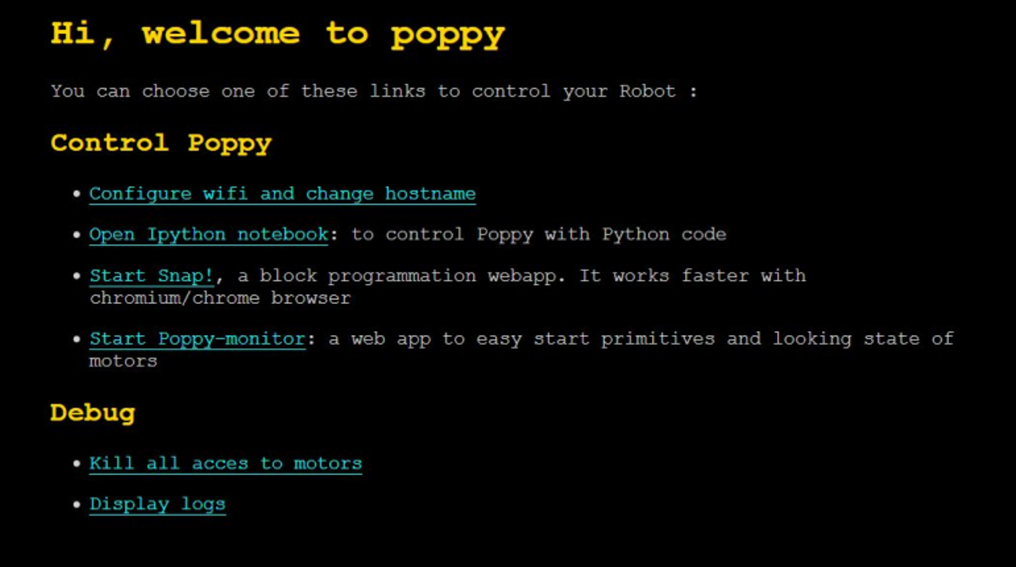
\includegraphics[width=\linewidth]{Figures/poppy_webhome-old}\label{fig:webhome_0}
                \subcaption{Version \textit{Alpha}, Segonds~\cite{RI}}
            \end{minipage}
            \hfill
            \begin{minipage}{0.475\linewidth}
                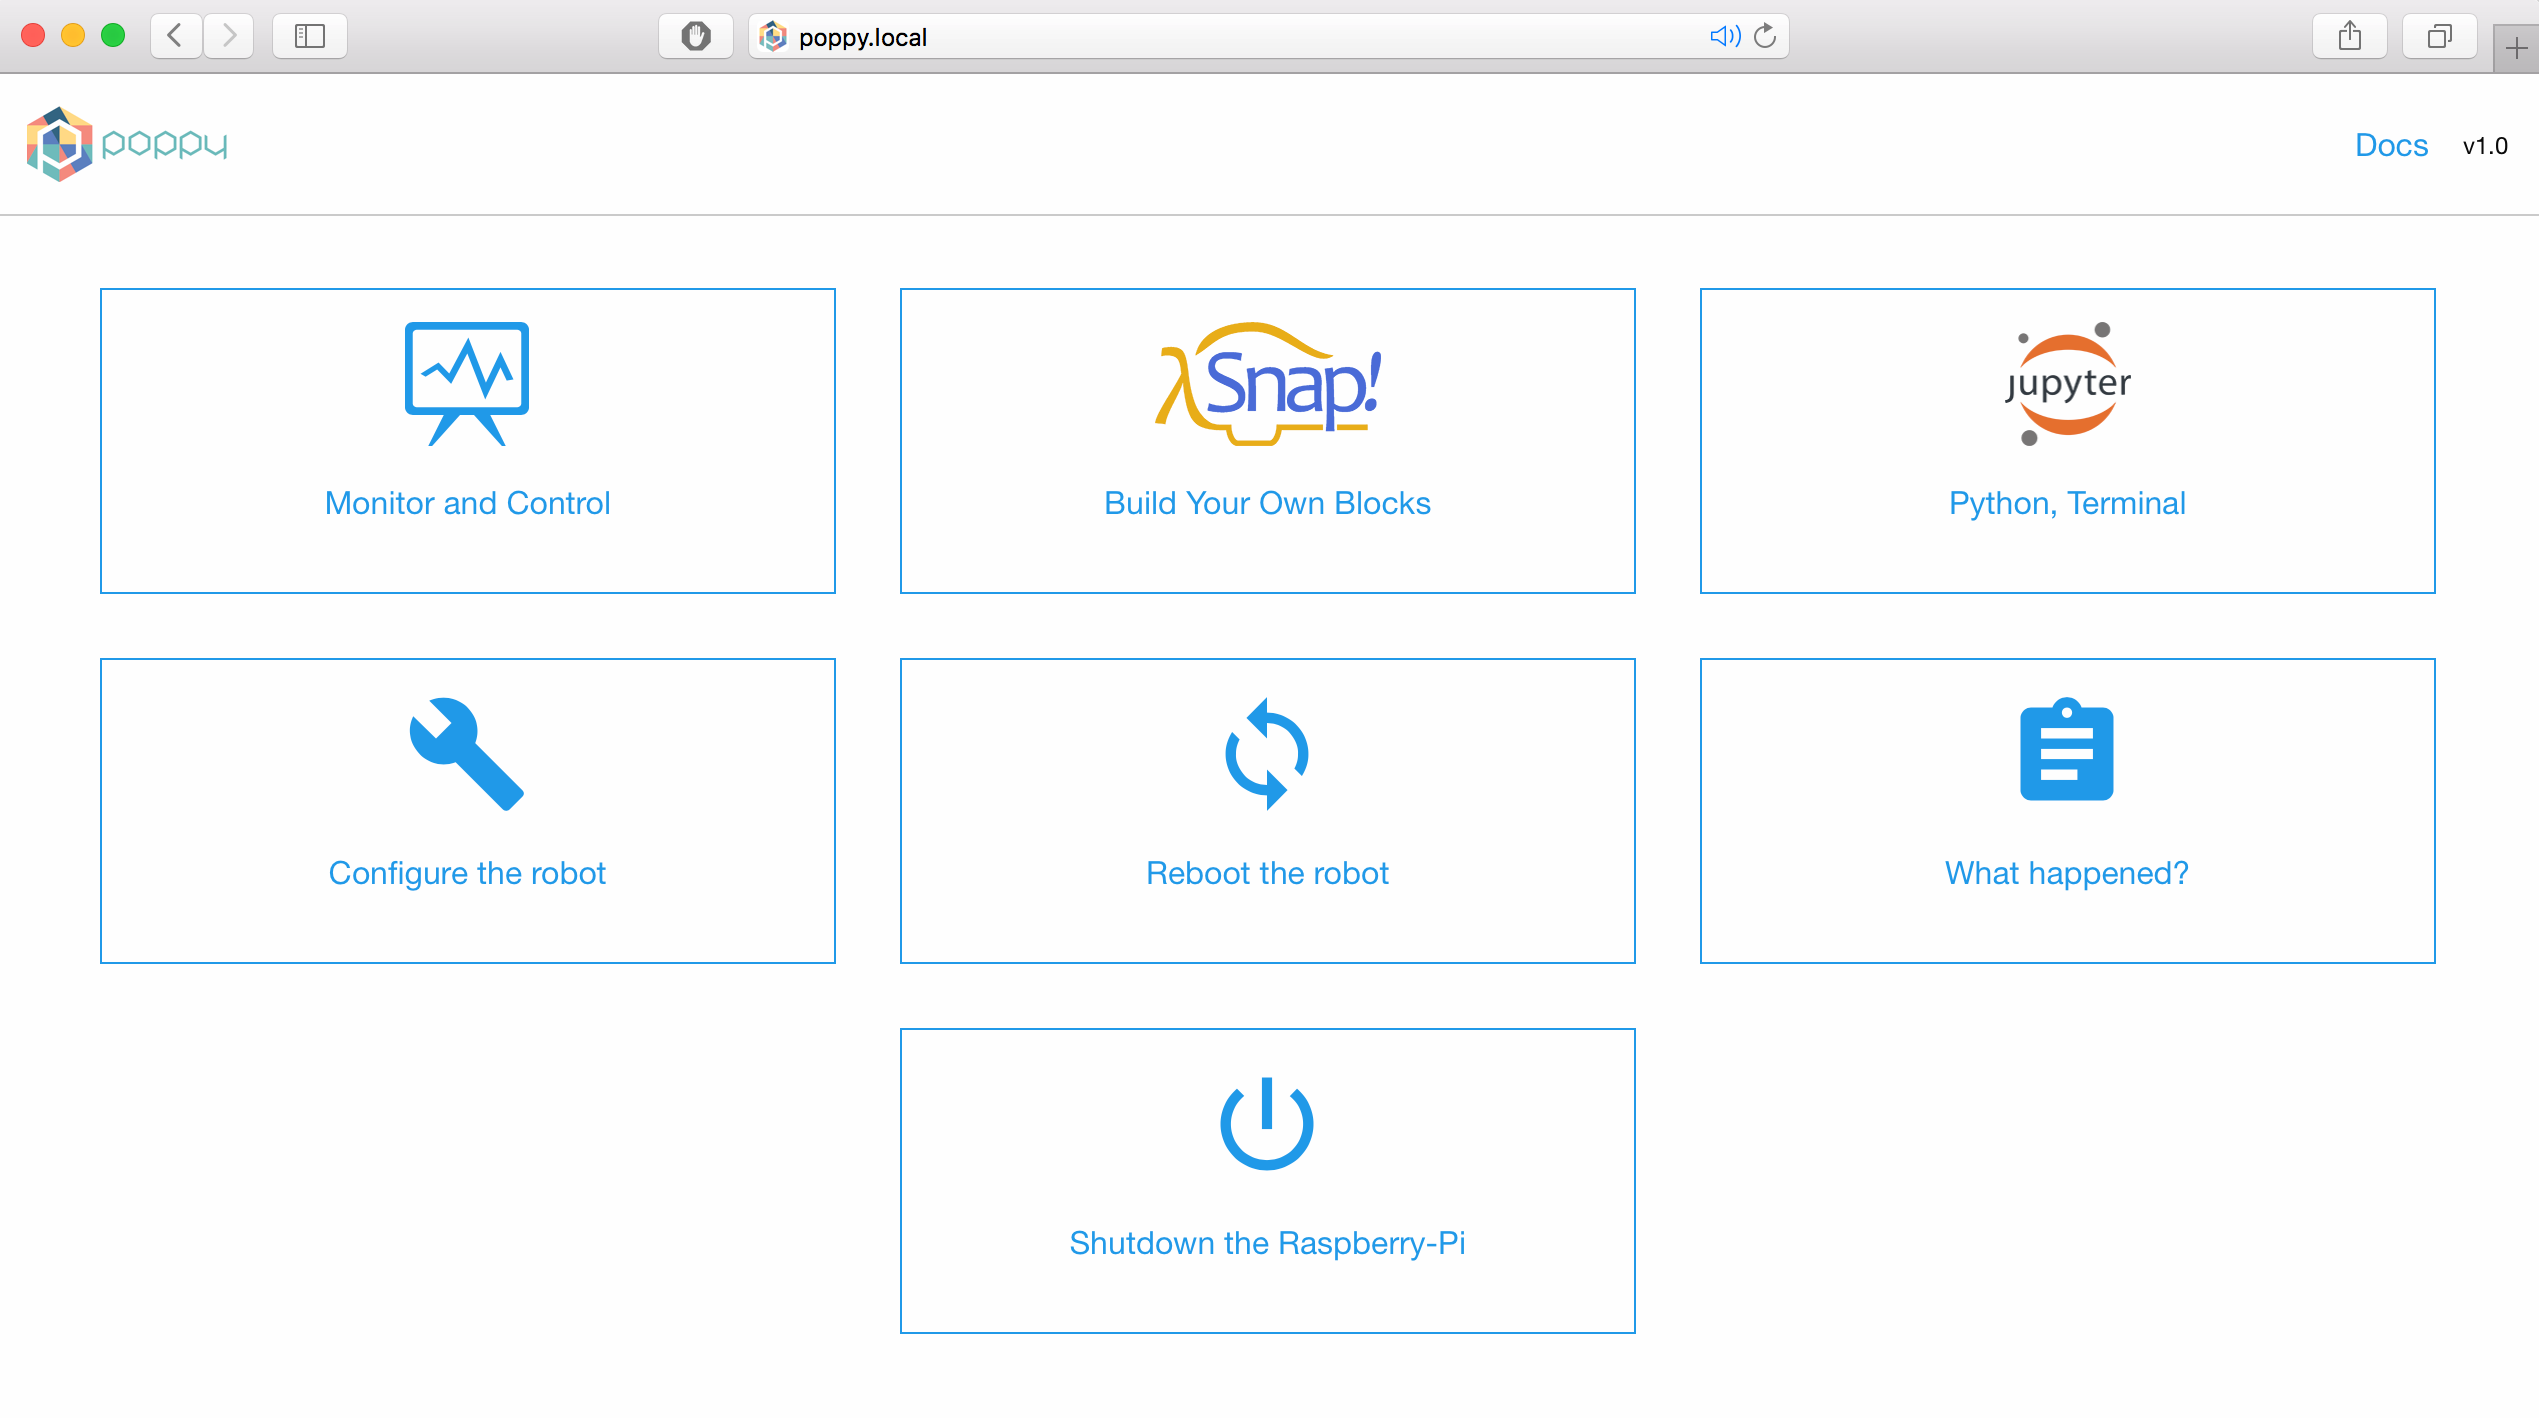
\includegraphics[width=\linewidth]{Figures/poppy_webhome}\label{fig:webhome_1}
                \subcaption{Version 1.0, Caselli~\cite{RI}}
            \end{minipage}
            \caption{Plateforme Poppy - WebApp Interface}
            \label{fig:webhome}
            \end{figure}\par%
            Elle se compose d'une bannière (comportant un lien direct vers la documentation) et de 7 encarts cliquables: 1 permettant la ré-instanciation du robot (qui s'exécute en python en \textit{background}); 1 permettant d'éteindre le robot; 1 autre pour sa configuration (moteur, wifi, \etc); un 4\ieme{} permettant d'afficher les \textit{logs} (issus de l'instance du robot s'exécutant en \textit{background}); enfin 3 encarts permettent respectivement d'atteindre: \cro{Poppy Monitor}, l'interface de programmation \sht{snap} et l'interface de programmation \sht{ipy}. Suite a plusieurs retours certaines améliorations sont en cours d'intégration pour une version 2.0.
        \paragraph{Programmation}\label{sec:programmation}
            \subparagraph{Poppy monitor}\label{sec:monitor}
                Une première manière de commander les robots Poppy est en utilisant une interface simple appelée \cro{Poppy Monitor} qui permet d’accéder à des comportements pré-programmés de haut niveau appelés primitives, ainsi que de visualiser l’état des capteurs du robot. Les primitives sont exécutées sous forme de thread. Chaque primitive possède une phase courante (qui boucle), une phase \cro{up} (au lancement) et une phase \cro{down} (à sa fin)~\citeS{sec:primitives}. Ces primitives sont rédigées en python et s'attachent automatiquement à l'instance du robot à son démarrage. L'utilisateur peut rédiger et intégrer ses propres primitives~\citeURL{TD-primitives} qui seront alors disponibles (entre autres) dans \cro{Poppy Monitor}.
                %La seconde est une interface de programmation visuel utilisant \sht{snap}. \sht{snap} est un langage de programmation graphique par blocs. Les blocs peuvent s’agencer ensemble pour former une suite d’instructions qui vont s’exécuter de façon séquentielle, et il est possible d’avoir plusieurs bout de code qui vont s’exécuter de façon concurrente, grâce à un ordonnanceur intégré.
            \subparagraph{ipython} 
                Il est aussi possible de programmer le robot en Python, en utilisant des notebooks Jupyter, une interface web permettant d’exécuter des cellules de code et d’en faire un document enrichi mêlant des images, du texte, des graphiques et du code. Cet interface permet donc à l'utilisateur de programmer le robot en Python en utilisant l'environnement d'exécution du robot, sans avoir à installer quoi que ce soit sur son ordinateur.
            \subparagraph{snap}\label{sec:snap_choice}
                Concernant cette dimension, aucune ligne historique émanant du Poppy-project n'est venue affecter le choix du langage de programmation visuel par bloc à visée éducative.
                Il en existait principalement trois: \sht{scra}, \sht{bloc} et \sht{snap}.
                \sht{scra} est un langage de programmation visuel développé dans le Lifelong Kindergarten au MIT Media Lab.
                Fort de 25 millions d'utilisateurs inscrits sur la plate-forme de partage de programmes en 2018, il est probablement le langage visuel par blocs le plus utilisé dans le monde. 
                Il a été pensé comme un successeur du langage Logo~\citeB{harel1990software}. Il se veut facile à aborder, mais aux possibilités très grandes.    
                Les blocs de \sht{scra} sont conçus comme des briques qui peuvent s'imbriquer entre elles selon leur fonction logicielle, cela permet aux enfants de commencer à bricoler avec et d'expérimenter sur le résultat produit, sans risque d'erreurs de syntaxe.
                Il est très simple d'utilisation, et le faible nombre de blocs disponibles en fait une force, le rendant très accessible aux plus jeunes.
                \sht{scra} 2.0 est utilisable en ligne dans un navigateur web avec Flash, ainsi que dans une application native multiplateforme qui nécessite d'installer Adobe Air.
                D'un point de vue purement technique, on peut reprocher à \sht{scra} 2 d'utiliser une technologie dépassée. Il nécessite l'utilisation de Flash pour fonctionner dans un navigateur, ou de Adobe Air pour s'utiliser de façon native. De plus, bien qu'il soit possible de rajouter des blocs personnalisés, ce système n'a pas été pensé à l'origine pour s'interfacer avec du matériel, ce qui le rend très peu pratique par rapport à ses concurrents sur ce point.
                De plus, l'équipe de \sht{scra} a toujours tenu à conserver un nombre de blocs très restreint. Leur volonté est de maximiser les possibilités qu'offrent ce langage avec un minimum de compréhension nécessaire pour l'utiliser.
                Certains contributeurs de \sht{scra} ont souhaité faire une version dérivée qui corrige selon eux ces deux problèmes, la limitation du langage et son utilisation dans un navigateur sans nécessiter Flash. C'est ainsi qu'est né \sht{snap}~\citeB{harvey2014snap}, anciennement appelé aussi BYOB (Build Your Own Blocs), mettant en avant la facilité de créer des nouveaux blocs dans le langage de bloc directement.
                Afin que les utilisateurs de \sht{scra} puissent l'utiliser sans nouvel apprentissage, \sht{snap} possède une interface très similaire en prenant un soin particulier à conserver les même blocs de base.
                En plus des blocs de base hérités de \sht{scra}, \sht{snap} possède des bibliothèques logicielles de blocs avec des fonctionnalités plus avancées, telles que des listes à compréhension, des éléments de programmation fonctionnelle et orientée objet, une interaction aisée vers l'extérieur grâce à son bloc http.
                \sht{bloc}~\citeB{fraser2014google} est conçu comme un logiciel de programmation par bloc extrêmement personnalisable. Il fonctionne majoritairement par traduction de bloc. On crée des blocs en leur donnant une signification dans un langage textuel, l'utilisateur compose les blocs de manière à former un programme. Lorsque l'utilisateur lance l'exécution du programme, cela traduit la séquence de blocs en un programme textuel spécifié par le développeur. La programmation par bloc est vue comme une étape pour se diriger vers la programmation textuelle, l'un étant une traduction directe de l'autre. Il ne permet pas dans son utilisation la plus courante d'exécuter plusieurs bouts de code en parallèle dans le même environnement comme cela se fait avec \sht{scra} ou \sht{snap}. Sa personnalisation en est toutefois sa force, il est aujourd'hui utilisé comme base pour la future et troisième version de \sht{scra}.\par%
                Nous cherchions une interface de programmation par bloc fonctionnant dans un navigateur et permettant les usages les plus vastes possibles pour ainsi rendre la programmation du robot accessible aux débutants, et de laisser aux personnes les plus à l'aise, le soin de le programmer et de le détourner dans des usages que nous n'avions pas prévus. C'est pour toutes ces raisons que nous nous sommes tournés vers l'utilisation de \sht{snap}.
                \sht{snap} est donc un environnement de programmation visuel par bloc fonctionnant dans un navigateur web~\citeB{harvey2014snap}. Il est conçu comme un outil d'initiation à la programmation et à l'algorithmique. 
                Inspiré fortement de \sht{scra}, il possède également un certain nombre de fonctionnalités plus complexes, comme des éléments de programmation orientée objet, des listes de listes, des éléments de lambda calculs ou des lutins récursifs. Ainsi, bien qu'il soit un très bon outil pour une première approche à la programmation, il permet également d'aborder des notions complexes et théoriques en s'abstrayant des problèmes de syntaxe que peuvent rencontrer des étudiants.
                Dans ce contexte, il est utilisé dans \textit{The Beauty and Joy of Computing}, un programme d'initiation à la pensée informatique pour les lycées et la première année de licence, développé à l'université de Berkeley~\citeB{garcia2015beauty}.
                \sht{snap} met à disposition un bloc \textit{http} qui permet d'effectuer des requêtes HTTP GET. Ce bloc est utilisé pour communiquer avec une API du robot, et ainsi le contrôler depuis l'interface de \sht{snap}. Nous avons développé des blocs personnalisés pour l'utilisation des robots Poppy. La création de ces blocs peut se faire en \sht{snap} lui même, ce qui permet aux étudiants de venir décortiquer et comprendre le code qui commande le robot.
                Le choix du nom des blocs est critique pour la facilité d'utilisation du robot. Il a fallu trouver un compromis entre la lisibilité des blocs et leur longueur dans le choix du vocabulaire. Ceci a été fait de manière itérative au cours du développement du robot, en organisant des ateliers et en observant les difficultés rencontrées par les enfants à la compréhension autonome des blocs.
\section{Les ressources pédagogiques}
    \subsection{Le site web}
        %cf aurelie lopez
        Sur le web, nous avons utilisé, dès le départ, la même architecture que Poppy-project (Github, forum, twitter, documentation, site poppy-project.org, youtube,Twitter, Flickr, \etc) en apportant quelques modifications pour les adapter à nos besoins (comme ajouter une partie \textit{Éducation} sur le forum, une page vitrine sur le site internet et un compte Twitter spécifique à Poppy Éducation~\citeURL{poppy-EduTwitter}). Puis, nous avons recueilli des retours d'enseignants partenaires par l'intermédiaire d'entretiens semi-directifs. Il en est notamment ressorti que les activités pédagogiques mises sur le forum étaient difficilement trouvables, l'accès aux ressources externes telles que la documentation était compliqué et que la langue anglaise rendait difficile la compréhension. Les réponses les plus données lors des entretiens étaient: \gui{les ressources sont difficiles à trouver, voire manquantes ou indisponibles en langue française}, \gui{la hiérarchie des informations présentes sur le forum est difficile à comprendre}, \gui{le contenu du forum est trop technique ou s'adresse à des utilisateurs avancés}, \gui{besoin d'avoir des activités à faire en classe, ou des idées pour les réaliser soi-même}.
        S'en est suivie une large restructuration de ce contenu; chaque activité réalisée en salle de classe étant désormais présentée et documentée sur une page internet dédiée sur le site web~\citeURL{poppy-Education}, avec sa fiche descriptive et toutes les ressources produites permettant de l'illustrer (photos, vidéos, productions d'élèves, \etc) et de la reproduire (fiche élève, fiche enseignant, corrections, \etc). Afin de permettre aux utilisateurs d'échanger sur l'activité, sur chaque page, un lien redirige vers un fil de discussion du forum Poppy-project \href{https://forum.poppy-project.org/c/Education/pedagogical-activities}{Poppy-project}.
        Pour les autres projets non scénarisés, une page vitrine \cro{démos} présente également des vidéos et tutoriels d'élèves et d'enseignants, accompagnée de projets \sht{snap} ou Python, illustrant ce qu'il est possible de faire avec le robot ErgoJr.
    \subsection{L'entre-aide sur le forum}
       ~\citeURL{poppy-forum}
        Suite à ces retours utilisateurs, nous avons donc créé une nouvelle vitrine adaptée aux besoins spécifiques de la communauté Poppy Éducation sous forme d'un site internet wordpress en langue française cité plus haut. %Les spécifications, élaborées lors d'un atelier impliquant les utilisateurs étaient \gui{Être en langue française}, \gui{Être agréable visuellement et convivial},  \gui{contenir des rubriques spécifiques à la présentation des robots et aux ressources pédagogiques}, \gui{mettre à disposition un espace dédié à la communauté}, \gui{proposer un espace d'aide comprenant les questions fréquemment posées}.
        Nous avons également amélioré l'utilisabilité du forum notamment en traduisant la rubrique \cro{Éducation} en français et en créant une sous-rubrique \cro{activité pédagogique}. Ainsi qu'en améliorant l'accessibilité vers la documentation (qui a aussi été revue \eg en la traduisant en français, et en améliorant la mise en page) et vers les \textit{post} déjà résolus.
        Le forum reste le lieu d'échanges principal et les activités mises par les utilisateurs sur celui-ci sont ensuite mises en avant sur le site internet. %Quant à twitter, alors qu'il semble peu utilisé par les enseignants, il semble majoritairement utilisé par les bidouilleur, les fablabs et les institutions éducatives. Il permet à la fois d'effectuer une veille des utilisations, de partager les productions et les dernières actualités.
    \subsection{Le livret d'activité}
        \paragraph{Composition} 
            Le livret pédagogique est composé de sept activités guidées abordant les notions de base en programmation (telles que la programmation séquentielle, les branchements conditionnels, les boucles, les fonctions, les variables, \etc) et en robotique (comme l'utilisation de capteurs et d'actionneurs) avec des défis \textit{ludiques} pour appliquer les connaissances. Ces défis visent plusieurs niveaux de difficulté afin que chacun réussisse à créer un programme simple tout en permettant aux plus avancés de le complexifier. Finalement, une dizaine d'idées de projets, de difficultés croissantes sont proposées.
            \begin{figure}[!h]
                \centering
                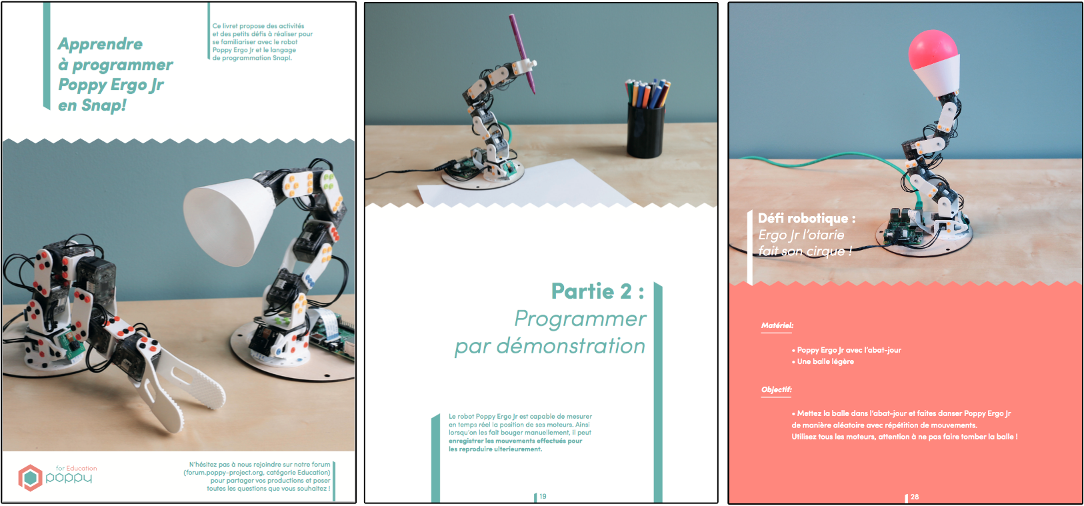
\includegraphics[width=0.9\linewidth]{Figures/Poppy-Livret_pedagogique}
                \caption{Livret pédagogique Poppy ErgoJr, Noirpoudre~\citeB{noirpoudre2016livret}}
                \label{fig:Livret_pedagogique}
            \end{figure}\par%
            Il présente également, en guise d'introduction, une définition de \textit{ce qu'est un robot} et présente les caractéristiques matérielles du robot Poppy ErgoJr ainsi qu'une partie \cro{commencer avec \sht{snap}} expliquant les points essentiels à connaître pour se connecter et utiliser l'interface. 
            Le livret n'est pas un objet \textit{fermé}, en effet ses possibilités sont étendues grâce à la catégorie \cro{activités pédagogiques} du forum du projet Poppy-project, un topic existe pour chaque projet et chacun est invité à le commenter et à partager ses productions. D’autant que de nouvelles activités sont régulièrement proposées par la communauté.
        \subparagraph{Processus de création}
            Quant au processus de création du livret pédagogique, l'équipe a conçu des premières ébauches d'activités, puis les enseignants volontaires les ont expérimentées en classe et ont fait des retours oraux, écrits ou vidéos. En parallèle, l'ingénieur pédagogique de l’équipe s'est déplacé dans les établissements partenaires afin d'observer la compréhension des différentes instructions, analyser les différentes manières d'interactions entre les élèves et le robot en fonction des personnalités et s'inspirer de leurs idées. Cela a permis d'améliorer les activités et de les adapter en fonction de la réalité de terrain et d'en créer de nouvelles. Par exemple, a émergé l’idée de petits défis ludiques.
            Ce cycle d'améliorations successives a été réitéré plusieurs fois avant de regrouper les activités en un livret pédagogique cohérent, accessible gratuitement en ligne.